\RequirePackage[l2tabu, orthodox, abort]{nag}
\documentclass[a4paper, 11pt]{article}

\usepackage[utf8x]{inputenc}
\usepackage[T1]{fontenc}
\usepackage{ucs}
\usepackage[english]{babel}
\usepackage{mathtools, amsmath, amsfonts, amssymb}
\usepackage{fancyhdr}
\usepackage[parfill]{parskip}
\usepackage{graphicx}
\usepackage[sc]{mathpazo}
\usepackage[scaled]{beramono}
\usepackage[scaled]{helvet}
\usepackage{float}
\usepackage{array}
\usepackage{booktabs}
\usepackage[font={small,it}]{caption}
\usepackage{fixltx2e}
\usepackage[colorinlistoftodos]{todonotes}
\usepackage{bm}
\usepackage{xfrac}
% \usepackage{fullpage}

\linespread{1.05}
\pagestyle{fancyplain}
\fancyhead{}
\fancyfoot[L]{}
\fancyfoot[C]{}
\fancyfoot[R]{\thepage}
\renewcommand{\headrulewidth}{0pt}
\renewcommand{\footrulewidth}{0pt}
\setlength{\headheight}{13.6pt}

\widowpenalty=1000
\clubpenalty=1000

\newcommand{\horrule}[1]{\rule{\linewidth}{#1}}
\newcommand{\vect}[1]{\mathbf{#1}}
\newcommand{\mat}[1]{\textbf{#1}}

\renewcommand{\thesection}{\uppercase\expandafter{\romannumeral 3}.\arabic{section}}

% Todonotes commands.
\newcommand{\addref}{\todo[color=red!40]{Add reference.}}
\newcommand{\rewrite}[1]{\todo[color=green!40]{#1}} 
\newcommand{\missing}[1]{\todo[inline,color=green!40]{Need to write: #1}}

\title{ 
\normalfont \normalsize 
\textsc{University of Copenhagen} \\ [25pt]
\horrule{0.5pt} \\[0.4cm]
\huge StatML: Exam 2014\\
\horrule{2pt} \\[0.5cm]
}

\author{Jens Fredskov (chw752)}

\begin{document}
\maketitle

\section{Predicting the Specific Star Formation Rate} % (fold)
\label{sec:predicting_the_specific_star_formation_rate}

\subsection*{Question 1}
Notes: we could also do regularization, and/or radial/polynomial basis functions.
Source code: question1.m linearRegression.m meanSquaredError.m

\subsection*{Question 2}
Notes: we should probably use a neural network :/
Source code: question2.m

$\sigma = \sqrt{1 / (2 \gamma)} \Leftrightarrow \gamma = 1 / (2s^2)$

% section predicting_the_specific_star_formation_rate (end)

\section{Stars vs. Galaxies} % (fold)
\label{sec:stars_vs_galaxies}

\subsection*{Question 3}

Source code: question3.m jaakkola.m crossValidation.m

\subsection*{Question 4}

\begin{figure}[H]
    \centering
    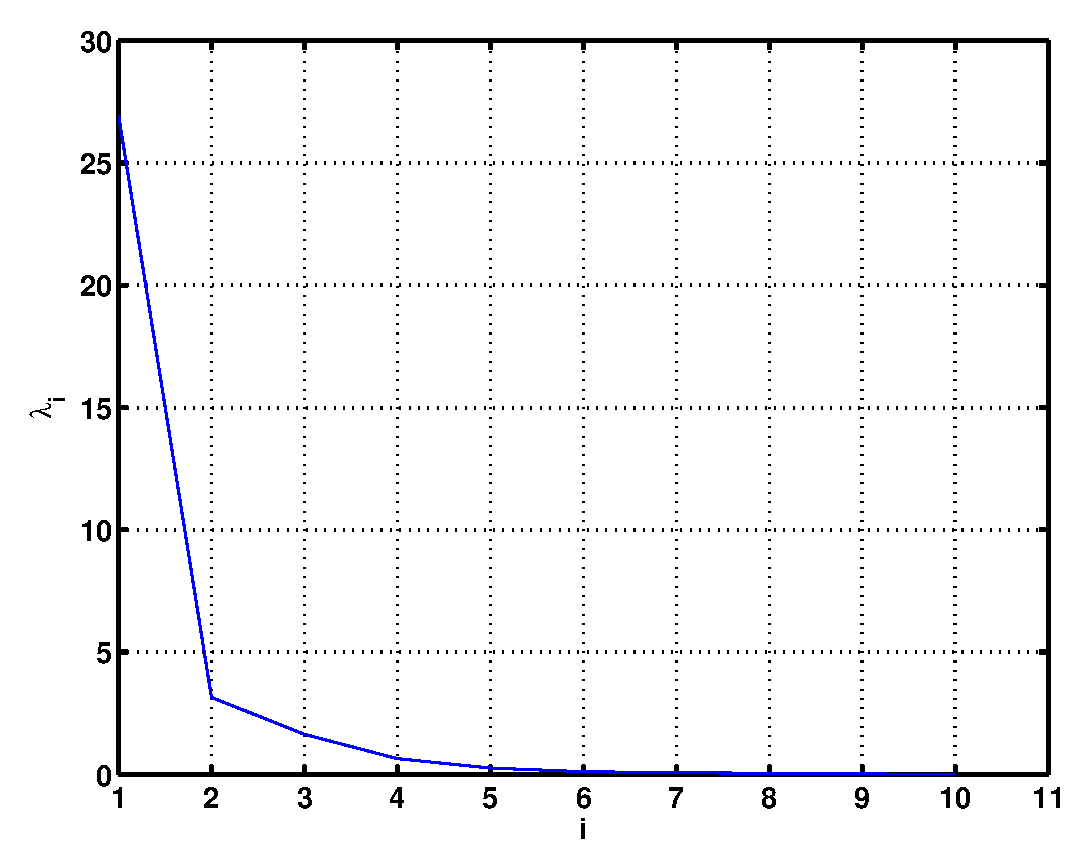
\includegraphics[width=0.8\textwidth]{figures/question4_1}
    \caption{Here be dragons.}
    \label{fig:question4_1}
\end{figure}

\begin{figure}[H]
    \centering
    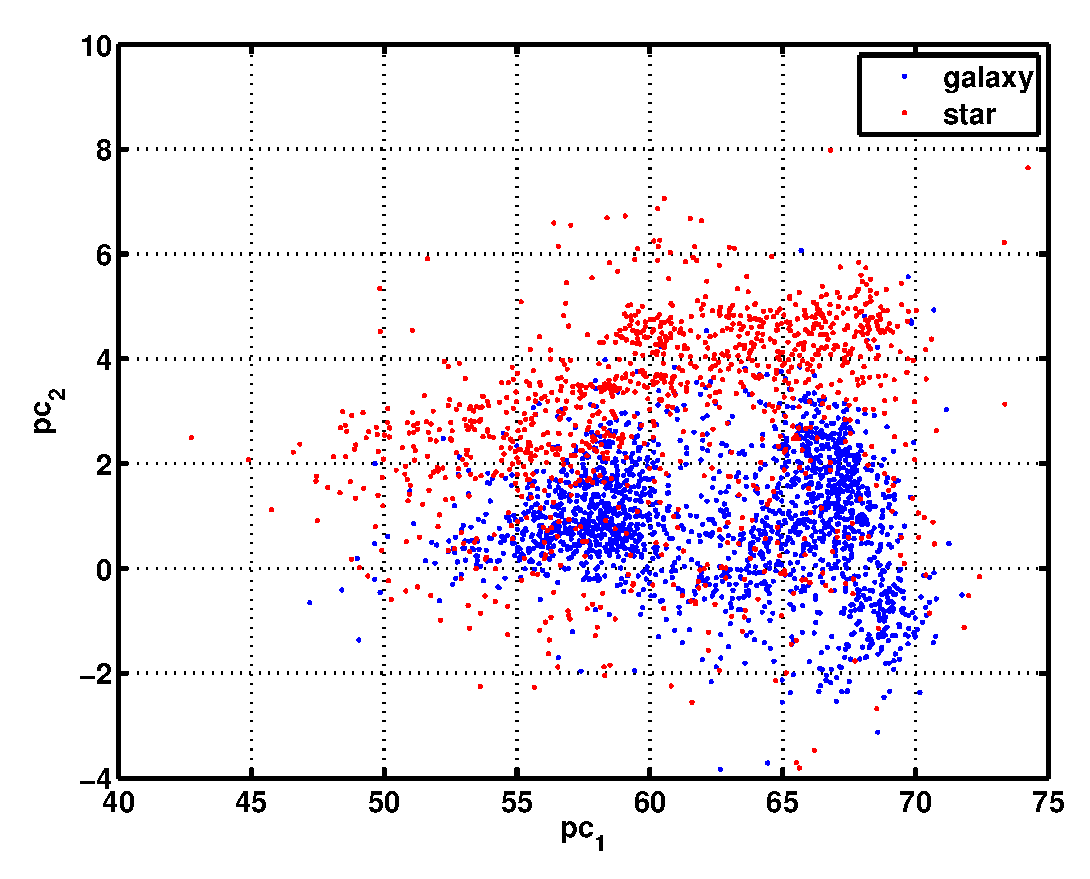
\includegraphics[width=0.8\textwidth]{figures/question4_2}
    \caption{Here be dragons.}
    \label{fig:question4_2}
\end{figure}

Source code: question4.m pca.m

\subsection*{Question 5}

\begin{figure}[H]
    \centering
    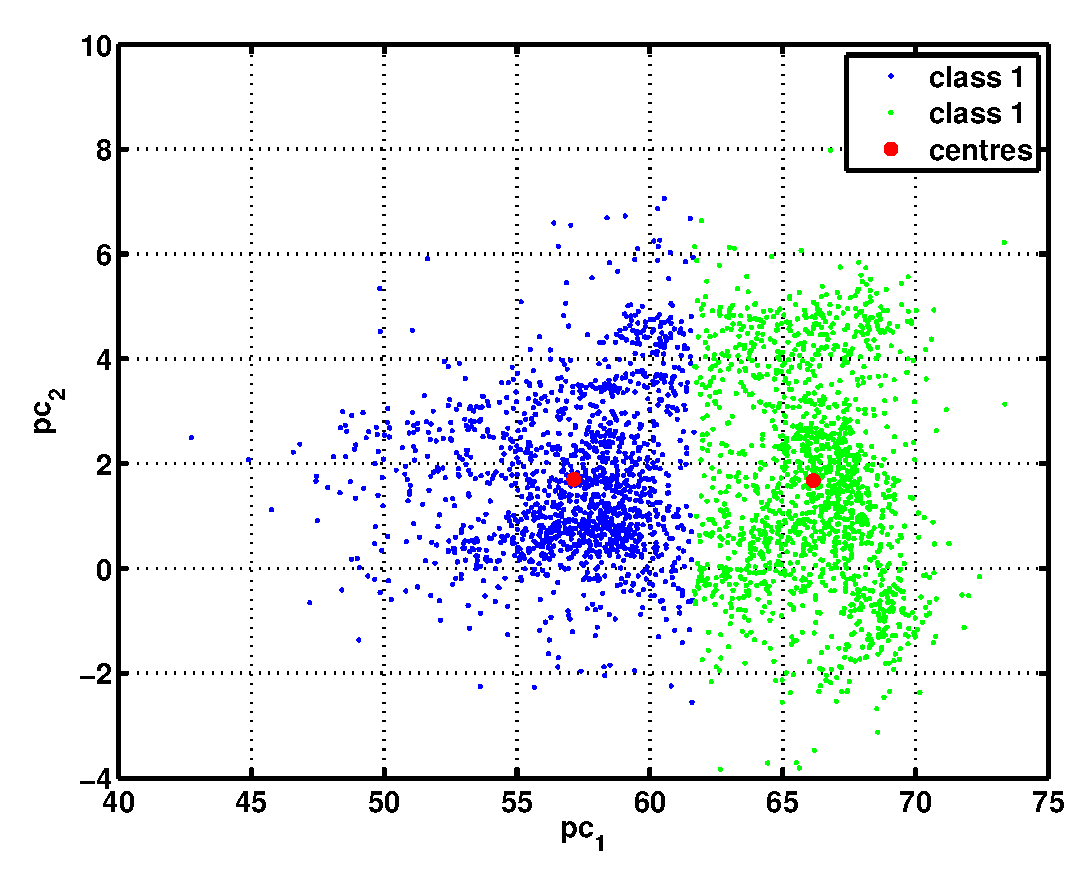
\includegraphics[width=0.8\textwidth]{figures/question5_1}
    \caption{Here be dragons.}
    \label{fig:question5_1}
\end{figure}

Source code: question5.m

\subsection*{Question 6}

% section stars_vs_galaxies (end)

\section{Variable Stars} % (fold)
\label{sec:variable_stars}

\subsection*{Question 7}

\subsection*{Question 8}

% section variable_stars (end)

\end{document}